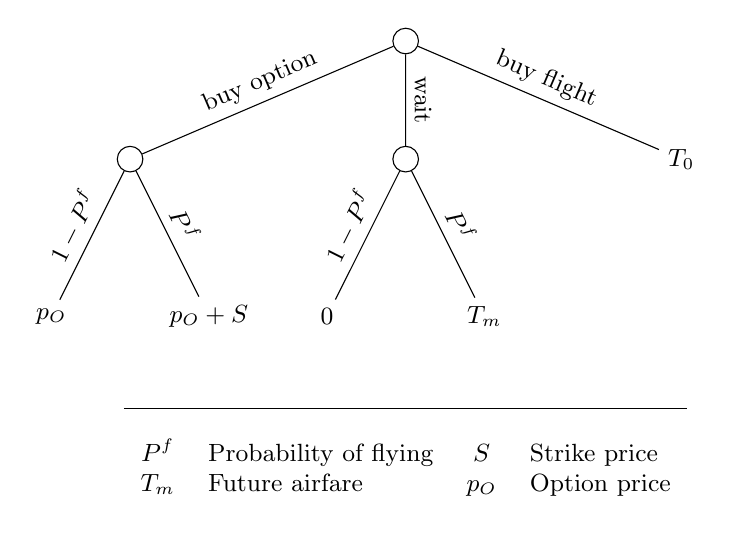
\begin{tikzpicture}[grow=down, sloped,
					level 1/.style={sibling distance=3.5cm, level distance=1.5cm}, level 2/.style={sibling distance=2cm, level distance=2cm},
					bag/.style={circle, draw, minimum width=1em}]
\small
\node[bag] {}
    child {
        node[bag] {}
        child {
                node {$p_O$}
                edge from parent
                node[above] {$1 - P^f$}
            }
            child {
                node {$p_O + S$}
                edge from parent
                node[above] {$P^f$}
            }
        edge from parent
        node[above] {buy option}
    }
    child {
        node[bag] {}
       		child {
                node {$0$}
                edge from parent
                node[above] {$1 - P^f$}
            }
            child {
                node {$T_m$}
                edge from parent
                node[above] {$P^f$}
            }
        edge from parent
        node[above] {wait}
    }
    child {
       node {$T_0$}
       edge from parent
        node[above] {buy flight}
    };

\node at (0,-5.25)
{
\begin{tabular}{clcl}
\hline \\
$P^f$ & Probability of flying &
$S$ & Strike price \\
$T_m$ & Future airfare &
$p_O$ & Option price
\end{tabular}
};
\end{tikzpicture}